\documentclass{lncs}
\usepackage[english]{babel}
\usepackage{graphicx}
\usepackage[numbers]{natbib}
\usepackage{amssymb,amsmath}
\usepackage{float}
\usepackage[cache=false]{minted}

\begin{document}

\title{To what extent can we utilise Semantic Analysis to realise emotional intelligence in machines}
\author{Stefan Starflinger BSc, Mag. Michael Walch, Prof. Dr. Dimitris Karagiannis}
\institute{Faculty of Knowledge Engineering, University of Vienna}

\maketitle
\begin{abstract}
Interactions between humans and computers have become common place. Although for robots to live alongside humans they need to possess some form of emotional intelligence. In this paper we looked at how we can utilize the information harvested from natural language processing (NLP), to determine someone's sentiment. We especially looked at how emotionally intelligent a machine can become. The goal of this paper is to maximise the emotional quotient \cite{colman2015dictionary} of a robot. Similar to the IQ the emotional quotient is a scale of how emotionally intelligent someone is. The first step was to have a knowledge base of emotions as done by \cite{borth2013large}.

The next step was to have scenarios created using a modeling procedure. These scenarios are depicted by a model. The user can create a scenario, which adjusts his environment to be in a specific state, depending on the user's mood. To be able to define scenarios it was necessary to create a Meta Model of the robots possible actions. The actions are then mapped to emotional values/moods from a knowledge base such as an ontology. This has been achieved using SEMFIS \cite{cs3473}, which helped us create an environment where users can define in what emotional state they have to be for an action from the robot to be made. For future work, only a subset of actions needs to be classified by the users and the rest will be inferred. Additionally, fuzzy sets were also considered as an alternative and/or an addition to an ontology. It was even considered to integrate fuzzy sets into ontologies \cite{calegari2006integrating}.

Finally, a validation environment was created with a subset of the specific case. To validate the scenario, a NAO robot was used. The microphone and the Software Development Kit (SDK) was used to capture audio clips and to communicate these clips to the Google servers via a REST API. The first response from the API (speech to text) would be used to send another request. The second request would return the overall sentiment of the previously sent text. The value was used by the NAO to adjust the current scenario where a scenario is the current state of all the IOT devices in the local environment.

At first, we discuss a future case, how interactions between humans and machines will be in the next 15-20 years. Then a generic approach of how we would achieve the described future will be discussed. The technology necessary for the advancement will be evaluated. A specific case will be looked at of what is already possible. And, finally, we validated if the case actually works.
\end{abstract}

\setcounter{tocdepth}{3}
\tableofcontents
\newpage

\section{Subject world}\label{sec:Concept}

To present the subject scenario in a more detailed and immersive manner I will narrate a short story depicting a potential future. This story will describe the interactions between humans and robots. Special attention should be placed on how the individual interactions play out, especially how the robot reacts to human endeavors. Consider closely what aspects are relevant and how the interaction between humans and robots can be improved. There will be two characters Alice a human girl and Bob her robot companion.

\subsection{Description}

Alice, a young slim girl at the age of 14 lives with her parents in the city. Currently, in the midst of her puberty, she has become very defiant. Her parents have trouble talking to her. She just has the feeling that no one understands what she wants. Stuck at home Alice is getting increasingly bored. The show she is watching in the living room does not satisfy the hole in her stomach. Her parents forbid her from going to her best friends birthday, who would do that, she thought.

Bob, her robot, and companion was very careful around Alice. He never tried to upset her, it felt to her like he knew how she was feeling, he knew what she was going through. Bob had been with the family for quite some time but never had Alice cherished the presence of him more. After the last software update, Bob had become increasingly pleasant to be around. Suddenly, a loud noise, Alice screamed. Her phone rang, which caught her completely off guard, pulling her out of her trail of thought. 

Bob was standing in his corner near the television and he could hear the caller trying to convince Alice to go out bowling. With hearing, his sensors i.e. his microphone picked up the sound coming from Alice' phone. Bob could not only hear the conversation but he could, thanks to the new software update, now also comprehend the underlying emotions of Alice that of her friend. His last software update gave Bob emotional intelligence on top of is artificial intelligence. Bob could now tell how upset Alice was, that her parents had not allowed her to go.

Moments after the call stopped, Alice turned off the television and left the living room. Bob would normally stay in his spot but today, he was worried. Would Alice do something stupid. Her emotional state was not normal and Bob knew Alice was less likely to behave rationally. Bob moved towards the door when he saw Alice putting on her jacket. "Where are you going?" Bob asked. "None of your business!" Alice replied in an angry tone, "If you're going to your friends let me come with you" Bob asked, trying to not upset Alice further. Bob knew if he upset her further Alice would just leave and he would have to call her parents. But by the time they would arrive Alice would be gone. "All my friends can leave home without taking their robot", she said while unlocking the door. "If you take me at least I can tell mom and dad afterward, that you were safe, the whole time", Bob said desperately. Then, Alice realized that she would be in a lot more trouble if she did not take Bob and replied "fine".

On their way to the subway, lots of robots pass them. Somewhere carrying their owner's bags, others were delivering packages. It would be a half hour journey to a distant district that Alice had not been before. Bob showed Alice the fastest route and once they got to the platform they left in the next Hyperloop capsule that arrived. On their way back out to the surface, a man in the elevator approached Alice. He wanted to sell her some product but she obviously did not want it. Bob could see that it made Alice uncomfortable and the man persisted, coming closer. Even though Alice had replied no thank you in a polite tone hiding her emotions because she was scared, the man did not want to leave. This is when Bob jumped in to defuse the situation. Reluctantly the man walked away.

Once Alice and Bob arrived at the destination address Alice told Bob seemingly excited "My friends should be somewhere inside". Alice and Bob were standing in front of a 43 story building with a big sign above the entrance spelling out 'bowling alley'. Unfortunately, Alice had no idea where in the building her friends would be. She tried to contact her friends but none of them were available. Bob could she that she was impatient and a bit scared. Bob needed to help so he contacted one of the robots of her friends and requested the robot to disclose the location of his owner (Alice friend) under the given circumstances(her emotional state). The robot analyzes the request and checks the relationship status between the two parties before submitting the floor on which Alice's friend is located.

Finally, Alice is with her friends, she seems delighted and happy. They play for quite some time, and the time goes by quickly. Bob reminds Alice after the third game that it is time to leave. Not only was Bob letting Alice disobey her parents but it is getting close to the curfew of Alice. She needs to be back home before midnight. After reminding Alice for the third time while it already being close to midnight Bob has no other choice than to contact Alice parents.

When Alice parents arrive, she is in big, big, trouble. Her mother is deeply disappointed. They take Alice and Bob home straight away. Alice has to promise her mother never to leave home without her parent's consent. They are very thankful and surprised that she at least took Bob with her to keep her safe. Bob was able to be a guardian for Alice without imprisoning her through analyzing her emotions and assisting her current state of mind to work towards a solution.

\subsection{Pepper - where we are today}

\begin{figure}%[H]
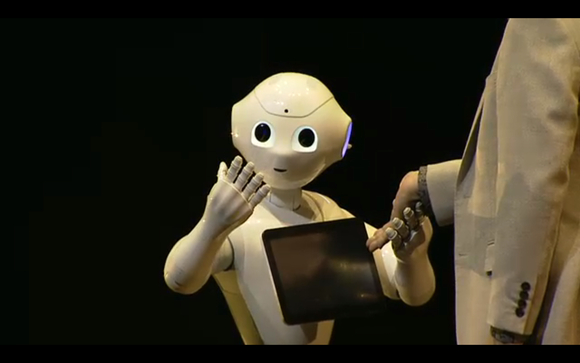
\includegraphics[width=\linewidth, height=6cm]{pepper.png}
\caption{Emotionally intelligent robot \cite{pepper}}
\label{fig:pepper}
\end{figure}

As we can see in figure \ref{fig:pepper} an emotionally intelligent robot named pepper is already being mass produced. A new era where robots need to learn to interact with humans is already upon us. Similar to the story told above, the robot interacts with customers in shops. Its goal is it to entice customers into the store and to help them with any questions they might have. Customers might be shy at first, and that is one difficulty that pepper needs to overcome. 

\section{Generic Approach}

%TODO: write about the theoretical concepts used, explain them in short sentences.
%export the model as xml with the ontology so it is machine readable
Human actions are not only powered by rationale but also by emotion, because of this, robots have to be emotionally intelligent. For robots to be successful in dealing with humans they have to align their actions according to the emotions of their owner, otherwise, a rather helpful robot can become a nuisance. Emotions can change how we view the world and our actions will adhere.
Currently, the digital world is based on true or false, one or zero. Emotions are far more complicated than that, a person can cry, because they are sad but on the other hand, they can also cry, because they are happy. This presents a unique difficulty in creating a knowledge base to accurately depict human emotions. A current practice to analyze the sentiment of someone is to perform a sentiment analysis on a bag of words. These are often texts composed in customer reviews, for a reseller to see and quickly respond to negative reviews. Although this is a good approach it is not the only one. Facial recognition and speech signal recognition as described in \cite{cowie2001emotion} by Cowie et al. can be used to analyze user emotion in human computer interactions. Another paper \cite{kim2004emotion} looks at how to create a system that can recognize human emotion through physiological signals, as facial expressions, for example, can be faked. As seen in the story, Alice did not show her true emotions to the stranger in the elevator. Finally, another paper \cite{borth2013large} looks into sentiment analysis using AI where different features in pictures disclose the emotion of the people depicted. Computer vision has come a long way and feature detection can help determine how a human is feeling as seen in figure \ref{fig:original}. An ontology has been \cite{borth2013large} created that can use computer vision to detect features and map these features to a mood. The ontology is primarily used for classifying the emotions of humans on pictures but in a sense, a video is nothing more than a series of pictures. This could enable a robot to 'see' emotion.

\begin{figure}%[H]
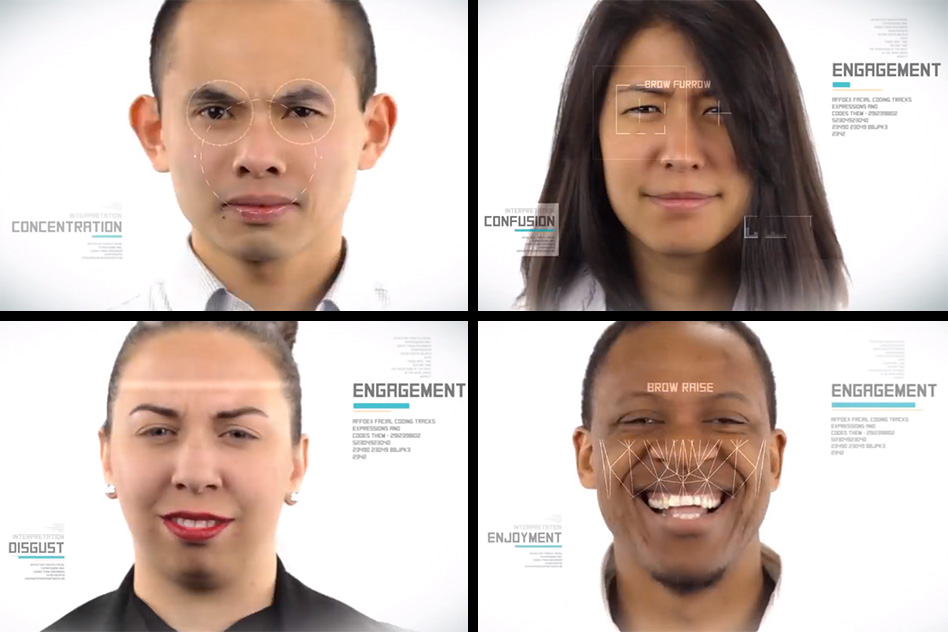
\includegraphics[width=\linewidth, height=8cm]{original.jpg}
\caption{Emotion recognition \cite{imagerec}}
\label{fig:original}
\end{figure}

In figure \ref{fig:original} we can see different faces and the features that are used to detect the different emotions. The emotions listed in the picture come from a knowledge base with many different atomic emotions.

Unfortunately, emotions are far from an exact science which makes it a difficult field to research. For example, sentiment analysis from a bag of words is difficult as presented in a paper from Bo Pang and Lillian Lee \cite{pang2008opinion} "If you are reading this because it is your darling fragrance, please wear it at home exclusively, and tape the windows shut." (review by Luca Turin and Tania Sanchez of the Givenchy perfume Amarige, in Perfumes: The Guide, Viking 2008). This sentence does not have any obvious negative words but its overall sentiment is negative. This shows us that sentiment analysis can be error prone. Meaning that in order to reduce the error, we could use a combination of different sentiment analysis techniques such as the ones described above. Because of the uncertainty of understanding natural language fuzzy sets as seen in figure \ref{fig:fuzzy} can be used.

Tapping into the emotional world has been accomplished by pioneers from Aldebaran Robotics. They have built a robot called pepper, as mentioned above, that can analyze human behavior. It is not actually too far away, or too unreasonable to assume that talking to a robot will be common place. Today, most of the intelligent assistants understand direct commands. The Amazon Echo among other devices has brought intelligent assistants to thousands of homes. These assistants are currently not aware of the user's emotions but can execute the commands they receive. A next step would be having an emotional assistant that is capable of understanding human emotion in order to execute commands accordingly.  Further, the intelligent assistant could execute different scenarios depending on the owner's emotion. When we are stressed or sad, we would not want there to be a lot of noise, so the robot/intelligent assistant should be quiet. It should not start the dish washer and it should not start the washing machine. What it should do is bring us some chocolate. If we are not feeling well the robot should make us a cup of tea.

Having a robot as an intelligent assistant e.g. a NAO at home will be like having a butler. He can run to different rooms, ensure everyone is safe and report anything suspicious. But, not only is the NAO interacting with the different devices inside of the house, he is interacting with the people that live there. For that, NAO needs emotional intelligence. For us to be able to make the NAO emotionally intelligent, we need a way for it to analyze and acts on signals e.g. the first step is converting sound waves into text. This is already one of the most difficult tasks for AI and falls into the AI-complete category. Not only is it necessary to identify which language, it is also necessary to identify the information correctly. The correct interpretation can be hard to find. Sarcasm among other language techniques is nearly impossible to detect. Each word in a sentence and its lexical meaning needs to be identified. After that, the semantics context needs to be determined. The NAO will not always interpret everything correctly. Giving the NAO fault tolerance and corrective mechanisms is essential. Of course, it is not necessary to have the lexical meaning of every word for the semantic analysis. It is rather the sentiment of each word that is needed. But since most systems run on commands, these commands need the lexical meaning. Having to solve the context and the sentiment increases processing. This has lead to centralized cloud solutions with light weight robot clients.

Next, we will look at the specific approach, where we will dive deeper into a more specific scenario in which a robot uses various classification algorithms to determine the mood of the user. Not only will the machine classify the mood but it will also act upon the results. Imagine being able to have a personal assistant that depending on how you feel always knows what to do. In this paper, we will look at scenarios that the user can create. The user will be able to model a scenario from a Metamodel and assign it with a semantic notation, which consists of a mood or a feeling. The robot can then execute a scenario after classifying the user's emotions. An example of a scenario would be modeling the lamps of an apartment and assigning different colors to those lamps depending on the semantically annotated mood. It would also be possible to connect individual colors to a mood. This brings us the specific approach.

\section{Specific Approach}\label{sec:specific_approach}

At the end of this document, there is a short section on definitions \ref{sec:definitons} that shortly explain what aspects need to be present for someone to be emotionally intelligent. It is our goal to express each of the points in the definition of emotional intelligence in robots. Firstly, "Monitor ones own and other people's emotion" we need to enable the robot to be aware of what emotions he is persuading and we need a system that can monitor other peoples emotions. To monitor others the robot will need sensors. To monitor the robots persuaded emotions he needs to be aware of what consequences his actions have. Secondly, "discriminate between different emotions" means the robot needs to be able to distinguish between someone who is happy and someone who is sad. Lastly, "use emotional information to guide thinking and behavior" means that the robot should act according to what emotions he perceives and persuades. Next, we will look more closely on how each of these three points can be accomplished.

As mentioned previously, there are multiple vectors from which it is possible to monitor the mood of a person. We will look more closely at deriving the mood through speech to text NLP and then performing a sentiment analysis on the text. Physiological and visual inputs will not be looked at. The use case would be, having someone talk to a robot. The robot would receive the input over sensors (microphone) as sound waves. It would then parse the waves to words creating a text. The text would then be analyzed using a sentiment analysis. Finally, the result of the sentiment analysis would be used to derive the membership value of the person having a particular emotion.

Through the influx of data, AI has been able to solve many problems. Using vast amounts of data, it is possible to apply deep learning techniques that can categorize almost anything. Combining machine learning with multi layered neural networks enables us to determine what the weight of a given input is. When a microphone picks up sound waves there is a lot of noise. This noise can be filtered to some extent, but with AI it has become possible to understand what word a certain sound wave represents to a high degree of certainty with or without noise.

We can determine how happy a person is depending on what he just said. Many customer service companies already use sentiment analysis in order to quickly react to bad reviews. As mentioned above, language is complicated and such sentiment analysis currently focuses mostly on sentiment polarity. This means, that we try and classify the sentiment of a bag of words to determine if it is positive or negative. Knowing the sentiment of someone does not necessarily mean that we know what mood they have. We do not have absolute knowledge about the person and there is a great deal of uncertainty. In order to have the most accurate results, a fuzzy set could be used. The fuzzy set could denote the membership of a sentiment in a given mood. For example, a sentiment of 1 would denote a high membership in the 'happy' set.

\subsection{Fuzzy Logic}

\begin{figure}%[H]
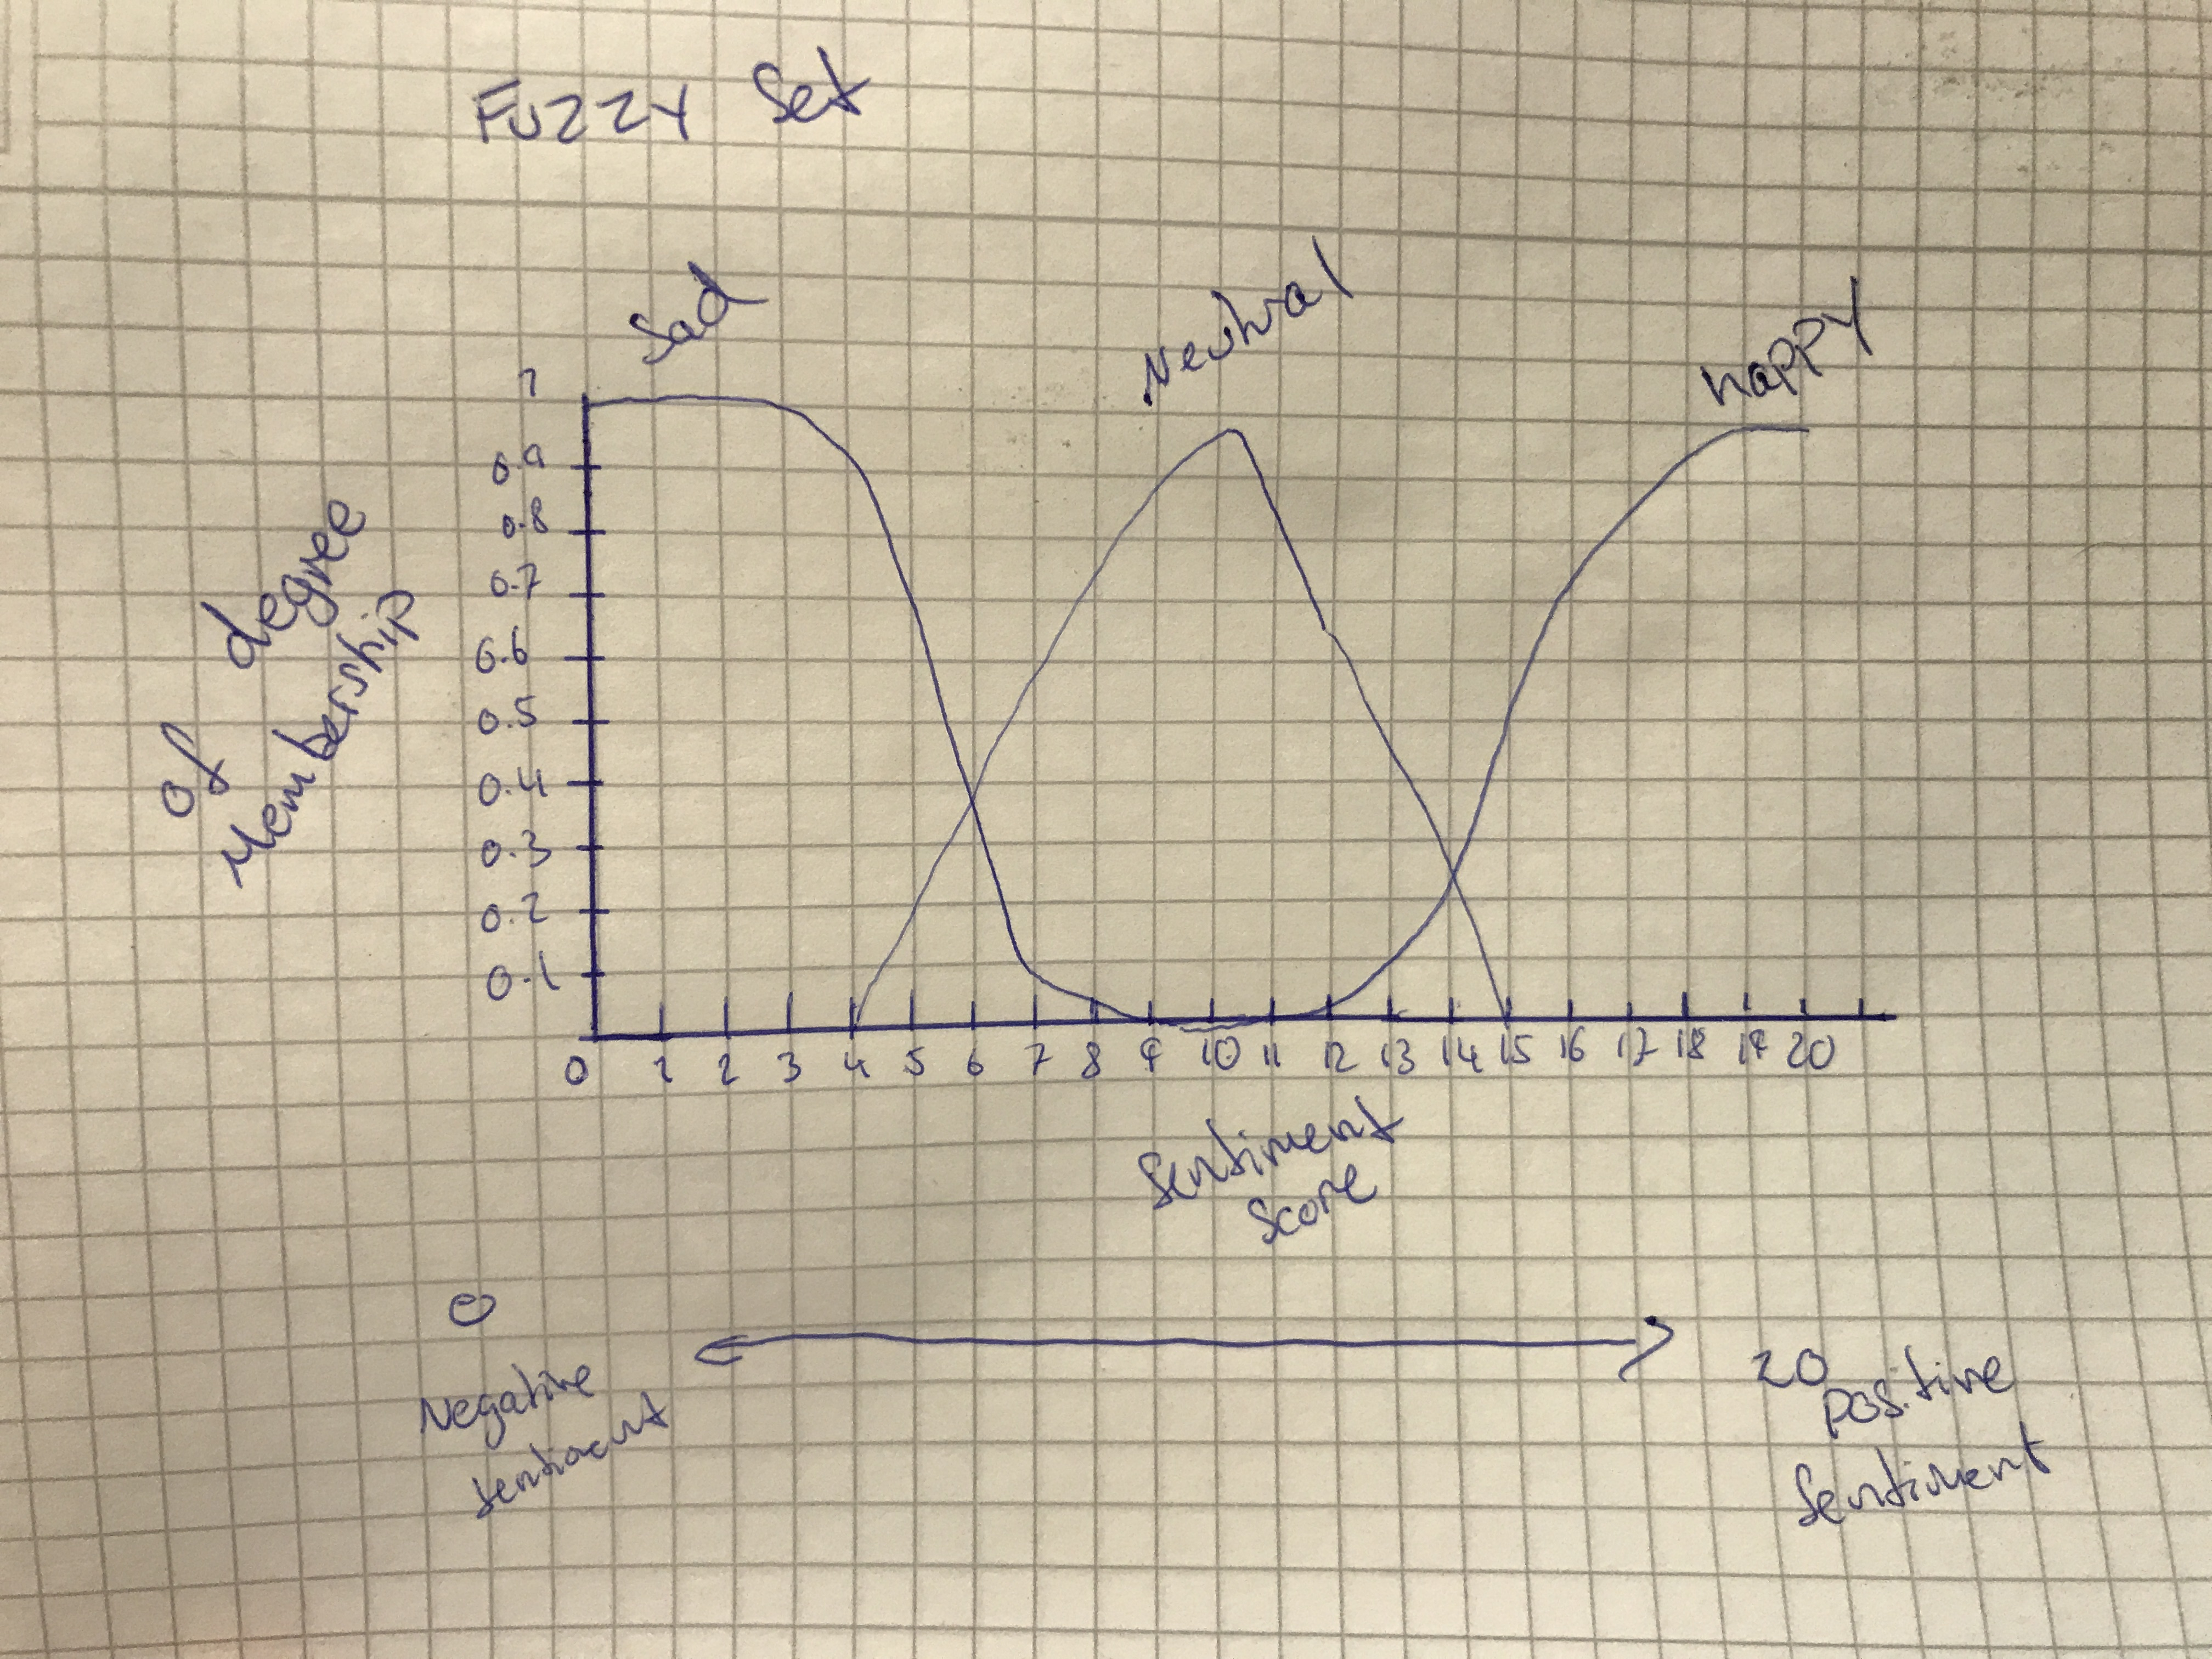
\includegraphics[width=\linewidth, height=8cm]{fuzzy.jpg}
\caption{Example of a fuzzy set}
\label{fig:fuzzy}
\end{figure}

As you can see in figure \ref{fig:fuzzy} there is a membership degree on the y axis and a sentiment score on the x axis. The 0 represents sad and the 20 represents happy. The scale is arbitrary and any other scale that is more convenient can be used. The names of the membership functions are displayed above. Sad to happy represents a sine curve and neutral crosses the sad and happy curve such as a cosine curve would. If someone were to have a sentiment score of 7 they would have a member ship in neutral at u=0.6 and a member ship in sad of 0.1.

In the analysis phase, once we have categorized different features and mapped them to an emotion we can act upon that emotion. A robot can be called emotionally intelligent once it can differentiate between different emotions. Using the concepts described above, we can analyze the sentiment of a person. With the sentiment, we can determine the membership of the person having a given mood. So we know the mood of the person, what the robot can then do is adjust its responses accordingly as well as adjusting the environment over the Internet of Things (IOT). If the membership were to be equal in two different groups it would be best if the robot did not do anything at all. This would mean that the membership has to be above a given threshold for the robot to act on the sentiment.

As we cannot guess what a person wants depending on their mood they need to be able to define different scenarios. These scenarios need to be configured beforehand and will determine what the robot executes when it detects a mood. Normally this would need constant supervision and monitoring. This seems far too complicated and a question such as "how are you?" or "how was your day?" should suffice for testing purposes for our specific case. The response to that question can determine the mood.

\subsection{Concept to Machine Layer}

\begin{figure}%[H]
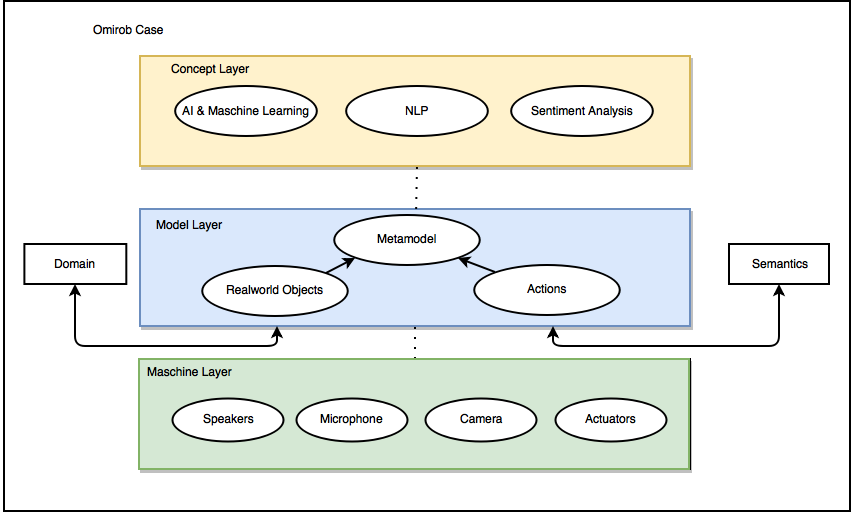
\includegraphics[width=\linewidth, height=8cm]{omirob.png}
\caption{Generic overview basis for the Specific approach}
\label{fig:concept-model-maschine}
\end{figure}

In figure \ref{fig:concept-model-maschine} we can see the concept layer at the top, the model layer in the middle and the machine layer at the bottom. To the left of the model layer, we can see the domain and to the right the semantics. The model layer is the center piece where everything comes together. Actions and real world objects are the things that the model depicts. The machine layer is connected to the model layer as the abstract objects that depict the real world can have these sensors or actuators. The Concept layer is connected to the model layer as it provides the model with algorithms and the general concept of what is being done. The meta model can have real world objects such as a robot or a person. These objects can then again have sensors. Further when the model interacts with the domain different actions can be described in the Metamodel that use algorithms from the concept layer to achieve an expected semantic result.

Although previously mentioned a fuzzy set would be used to categorize the mood of a person it does not necessarily prevent us from also using an ontology for inferences. We can declare a certain membership threshold at which an ontology knowledge base can be used to infer knowledge. For example, if a guest is sad, the ontology can infer that everyone else is also sad.

A Metamodel can be used to make scenarios available for the user to create. Not only can the Metamodel be used for the static implementation of scenarios but also for the connection of the NLP algorithms with the robot. Modelling procedures as seen in \cite{cs3657} can be used to enable easy creation of scenarios. The Metamodel would denote the possible actions as well as visualizing the environment in which the robot is in. Modeling procedures could combine semantics with models using SEMFIS \cite{cs4933}. More on that below.

\section{Validation}\label{sec:Validation}

We now come to an instance of what we described in the specific approach. We will look at how we can deploy such a use case in the real world today. The idea is to have a robot, the NAO interact with a human. To limit processing and to make validation easier the robot will be asking a question and will listen for a fixed amount of time. Once the robot is done listening, he analyses the sentiment and acts. All of this can be controlled via a model. The model can create scenarios that define the actions a robot does depending on the detected mood.

\subsection{Speach to text}

The biggest problem with doing AI yourself is that most of the time you do not have the huge amounts of data necessary. Since gathering vast amounts of data is very difficult, we will be using Google's speech and natural language processing (NLP) API. The latter will be used to convert sound waves to text and the other will be used to analyze the sentiment of the text. Since we are using Google's API, we can assume that the great amount of data Google has available will improve the accuracy of our results.

The NAO robot will be responsible for managing the smart home of a home owner. The robot will be able to interact with the user and ask him questions. With the answer to the questions, the robot will change the state of the smart home objects. We will look closely at how we should change the state of the home objects, according to the sentiment of the user.

Different scenarios can be modeled using modeling procedures. The home owner can create a model instance and denote the instance with a mood. This instance will be activated once the robot detects the mood. Multiple scenarios can be created in order to cover every possible sentiment.

\begin{figure}%[h]
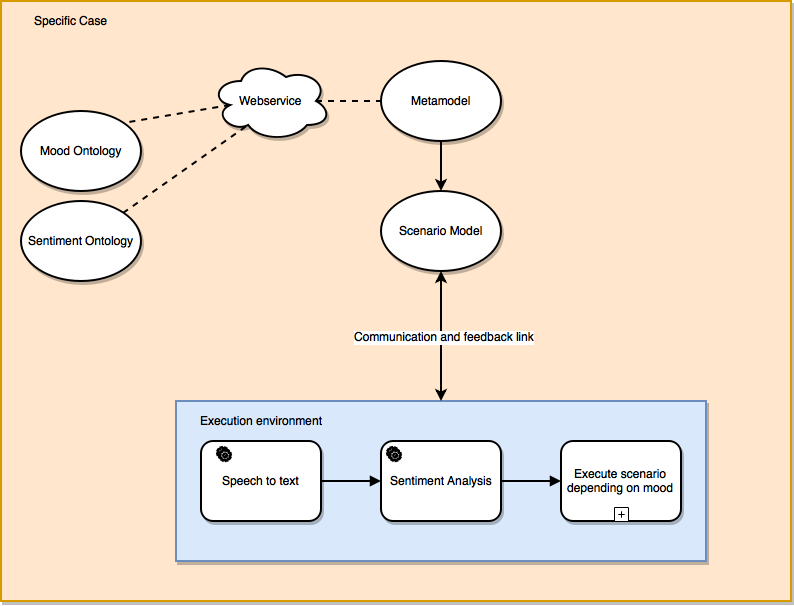
\includegraphics[width=\linewidth, height=7cm]{validationOmiRob.png}
\caption{Specific approach}
\label{fig:validation}
\end{figure}

In figure \ref{fig:validation} we can see how the model interacts with the execution environment. Further, we can see that the semantic annotations are not incorporated directly into the Metamodel but rather are available over a Webservice. This service enables us to easily change the ontology without having to change the Metamodel. It also lets us apply the ontology to many different models as it is independent.

The execution environment depicts two services that are executed remotely and a task that is executed locally. The services with a small icon on the top left are the remote services. The scenario model is an abstract model of the real environment. The user can connect instances of webservices to that environment. Furthermore, instances of IOT devices can be connected to the robot and their state can be set according to a specified mood. The webservice is not connected to the scenario directly as a web service entity should be created in the meta model. Although this is prone to errors when the endpoints change it is easier for the user to setup and safer for the API keys as the Metamodel handles these. This means that the API key cannot be modified or viewed by anyone who is working with the scenario model.

\subsection{Step by step}
The goal is to create an emotionally intelligent robot that understands the speaker's mood and adjusts the surroundings accordingly. As an example the mood will be projected through the use of lights, changing the color of the lights depending on the mood of the user. In this project, we will be using a NAO robot as our input device. The NAO robot runs on a Unix operating system, a version of linux. A program that will run on the operating system to control the NAO robot will enable us to interact with the user. The first step for the NAO robot would be to ask a question to start the conversation.

The NAO robot will ask the question "How are you" it will give the person 10-20 seconds to answer. After 20 seconds it will cut off the answer and start the sentiment analysis. The recording of the 20 seconds of text will be sent to the google speech API and then forwarded to the google NLP API in order to get the sentiment of the text. Using the sentiment score of -1 to 1 a lookup will be made using either a knowledge base or a fuzzy set. The given mood or the member ship will be retrieved.

First, we need to have sensors. We will need a microphone that can record sound. This microphone can be integrated into a robot such as the NAO. As stated the NAO will be running on a Unix distribution. This means that we need a microphone that supports software for a Unix system. The NAO robot has multiple microphones that are accessible over the robots SDK. Using the SDK then, we can record audio. The audio might need to be converted, depending on the format that the NAO robot uses. Not only does the robot need a microphone but it needs to start recording when the NAO is spoken to and start processing seconds after the person stops speaking. Further, the NAO bot needs to be connected to the internet.

\subsection{Google API}
So now, once an audio clip is recorded and in the right format, we can send it to Googles API for processing. The API can be found on the google cloud service called "Cloud Speach". Google offers a REST API with a speech.recognize call. The call looks like this:

A HTTP POST request needs to be made to this address: \\ \\ https://speech.googleapis.com/v1/speech:recognize \\ \\

and the body that has to be sent from the NAO bot should look like this:

\begin{minted}{json}
{
  "config": {
      "encoding": "FLAC",
  	  "sampleRateHertz": 44100,
      "languageCode": "AT",
      "speechContexts": [
	    {
	      "phrases":["Leiwand"]
	    }
	  ]
	  },
	  "audio": {
	    "content":"U29tZSBieXRlcyBhcyBhIHN0cmluZyBiYXNlIDY0IGVuY29kZWQ="
	  },
}
\end{minted}

There are two parts one is the RecognitionConfig file and the other is the Recognition audio. The config specifies how exactly the request should be processed and the audio specifies what is to be processed. There are a few optional parameters that are not mentioned above. The most important parameters that need to be present are listed above. The content variable \\"U29tZSBieXRlcyBhcyBhIHN0cmluZyBiYXNlIDY0IGVuY29kZWQ=" \\ is "Some bytes as a string base 64 encoded". This is not actually a FLAC encoding but just used as an example. The world 'Leiwand' can be manually added to assist the API. Some words are unusual and if phrases are added the Speech API can translate the phrase correctly.

The return value would look something like this:


\begin{minted}{json}
{
  "results": [
    {
      
      "transcript": "Some bytes as a string base 64 encoded Leiwand",
      "confidence": 0.9,
      "words": [
        {
            "word": "Some",
        },
        {
            "word": "bytes",
        },
        {
            "word": "as",
        },
        {
            "word": "a",
        },
        {
            "word": "String",
        },
        {
            "word": "base",
        },
        {
            "word": "64",
        },
        {
            "word": "encoded",
        },
        {
            "word": "Leiwand",
        },
      ],
    }
    
  ],
}
\end{minted}

After receiving the transcript we can now perform a sentiment analysis. One can see that we already have a means to retrieve and create a bag of words. We can either take the transcript or we can take the words array. An important value is the confidence, it tells us how successful the conversion is. Based on that value we could start over to ensure the robot has understood the person correctly. The sentiment analysis will again be done with the Google Cloud Platform. The NLP API of Google will look at the text and identify the emotional opinion in the text. An example of a request would look like this: 

\begin{minted}{json}
	{
	  "encodingType": "UTF8",
	  "document": {
	    "type": "PLAIN_TEXT",
	    "content": "Enjoy your vacation!"
	  }
	}
\end{minted}

Here we can see that in the body we need to specify the type of document, the content that is being analyzed i.e. our transcript from the previous response and the encoding type of the document. The response we would get from the sentiment analysis would look like this:

\begin{minted}{json}
{
  "documentSentiment": {
    "magnitude": 0.8,
    "score": 0.8
  },
  "language": "en",
  "sentences": [
    {
      "text": {
        "content": "Enjoy your vacation!",
        "beginOffset": 0
      },
      "sentiment": {
        "magnitude": 0.8,
        "score": 0.8
      }
    }
  ]
}

\end{minted}

Here we can see the overall 'documentSentiment' but also the sentiment of individual sentences. The score tells us how positive, up to 1 or how negative, up to -1, the sentiment is. The magnitude score, on the other hand, shows the total emotion positive and negative summed up together as a positive integer. This means that a sentence with an overall sentiment of -0.5 and 0.5 would have a score of 0 and a magnitude of 1. The score and magnitude occur twice in the response. The first time they are for the whole text and the second time the values are for a single sentence. We only have one sentence so the magnitude and score values are the same. Taking the score value and using the figure \ref{fig:fuzzy} we can determine the membership value. The sentiment value needs to be changed from -1 to 1, to 0 to 20 in order to fit the scale as seen in the diagram. The sentiment of 0.8 would be equivalent to 18 on figure \ref{fig:fuzzy} and give us a membership of 100\% in the happy set.

All of the code examples were taken from the Google Cloud Platform \cite{googlecloud} and modified as needed. An alternative to the google cloud platform would be the open source project Kaldi \cite{Povey_ASRU2011}. Kaldi is written in C++ and offers an Automatic Speach Recognition (ASR) software.

So far we have our platform the NAO robots, we have our NLP and we have our sentiment. What is still missing are the scenarios and the semantics of our emotions. In other words, the actions that the robot needs to perform once the sentiment value is received and what it means for the other people that are around. The scenarios will be created through a modeling procedure described below.

\subsection{Metamodeling}

A Metamodel that allows the user to map actions of the robot to moods resulting from a previously described sequence of events. These actions will consist of a model that displays a room of a house that contains smart home devices. These devices, in our case lamps have a range of possible states. The states can be modified through a central interface such as the NAO robot. The NAO robot is be wirelessly connected to the smart home objects. The states of the smart home objects can be denoted with a semantic meaning. The NAO robot can then change the state of a such a device after deriving the mood of the inhabitant, depending on what he responded to the question "How are you". For example, the user can set the mood of the color red to happy. This means that every time that the user is happy the color of the lights will be red. To do this the user would connect a mood element in the model with the IOT device. Then the user would set the color of the IOT device. This state will be activated every time the user portrays the specified mood.

The Metamodel is be connected to an ontology over a Webservice. This is a decoupled approach and lets us change the ontology without having to change the Metamodel. SEMFIS uses modern standards such as OWL and tools like Protege developed at Stanford University \cite{cs3473}. This means, that already developed ontologies can be used under the standard exported to XML and connected to the Metamodel elements. Similar to the ontology described in \cite{borth2013large} I have developed an ontology mapping features of actions to moods. This ontology can be used to determine what emotions the actions provoke in order for specific actions to be taken that align with a persons mood and not contradict it.

\subsection{Scenario Model}

%Image of a model that depicts a home together with semfis
\begin{figure}%[H]
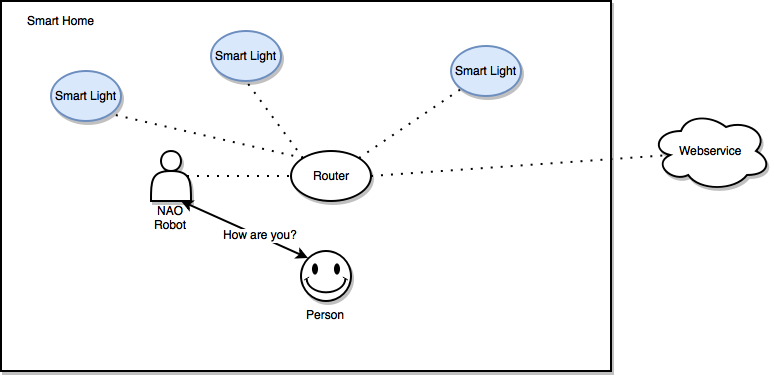
\includegraphics[width=\linewidth, height=6cm]{home.png}
\caption{Scenario Model Example}
\label{fig:home}
\end{figure}

In figure \ref{fig:home} we can see an instance of a model. This model uses dynamic graph rep \cite{cs3657} to display the color of the lights as well as the mood of the user. The NAO robot is connected to the smart home via a router that relays all of the commands to the smart objects in the house. In our case, the smart objects are the smart lights. The router also enables the NAO robot to connect to a Webservice. This lets the NAO robot to communicate with the Google API's as well as get information from ontologies. The individual lights can be selected with a query language in the model. Once selected the light can be controlled through the model.

\section{Conclusion}

In conclusion, we have created a validating environment that checks whether or not The NAO robot is emotionally intelligent in his actions. If the validation environment runs multiple test cases and each of them succeeds then the validation method would also be a success. The test cases should not require humans to monitor the system but a pre-defined test set with an estimated sentiment polarity should be used to see if the system is operational. Further, the system should validate the resulting state of the IOT devices with the Graphrep representation in the Model. As we can see from the paper, we are not too far away from having a fully functional robot that can interpret our emotions. The difficulty comes in having to ensure that the interpretation is correct.

In the future, it would be interesting to see what other devices in our environment could be controlled by our emotions. IOT in the future allows for everything to change without the user directly interacting with the system. The NAO bot could detect if the person was cold and adjust the heating.

\section*{Definitions}\label{sec:definitons}
\begin{itemize}
  \item emotional intelligence - "Ability to to monitor one's own and other people's emotion, to discriminate between different emotions and label them appropriately, and to use emotional information to guide thinking and behaviour." \cite{colman2015dictionary}
  \item this encompasses the ability to:
  \begin{itemize}
    \item perceive, appraise, and express emotions accurately
    \item access and evoke emotions when they facilitate cognition
    \item comprehend emotional messages and to make use of emotional information
    \item regulate one's own emotions to promote growth and well-being.
  \end{itemize}
  \item emotional quotient - "An index of emotional intelligence analogous to the IQ index of conventional intelligence." \cite{colman2015dictionary}
\end{itemize}

\nocite{*}
\bibliographystyle{natdin}
\bibliography{Bibliography}

\end{document}
